% !Mode:: "TeX:UTF-8"

\chapter{Reparameterization Trick}

\section{为什么需要Reparameterization}
当我们需要优化的系统中有一个从某个分布采样得到的样本作为另一个函数的输入,这个不确定的采样得到的样本使得梯度回传存在问题, 如图:
\begin{figure}[htbp]
\centering
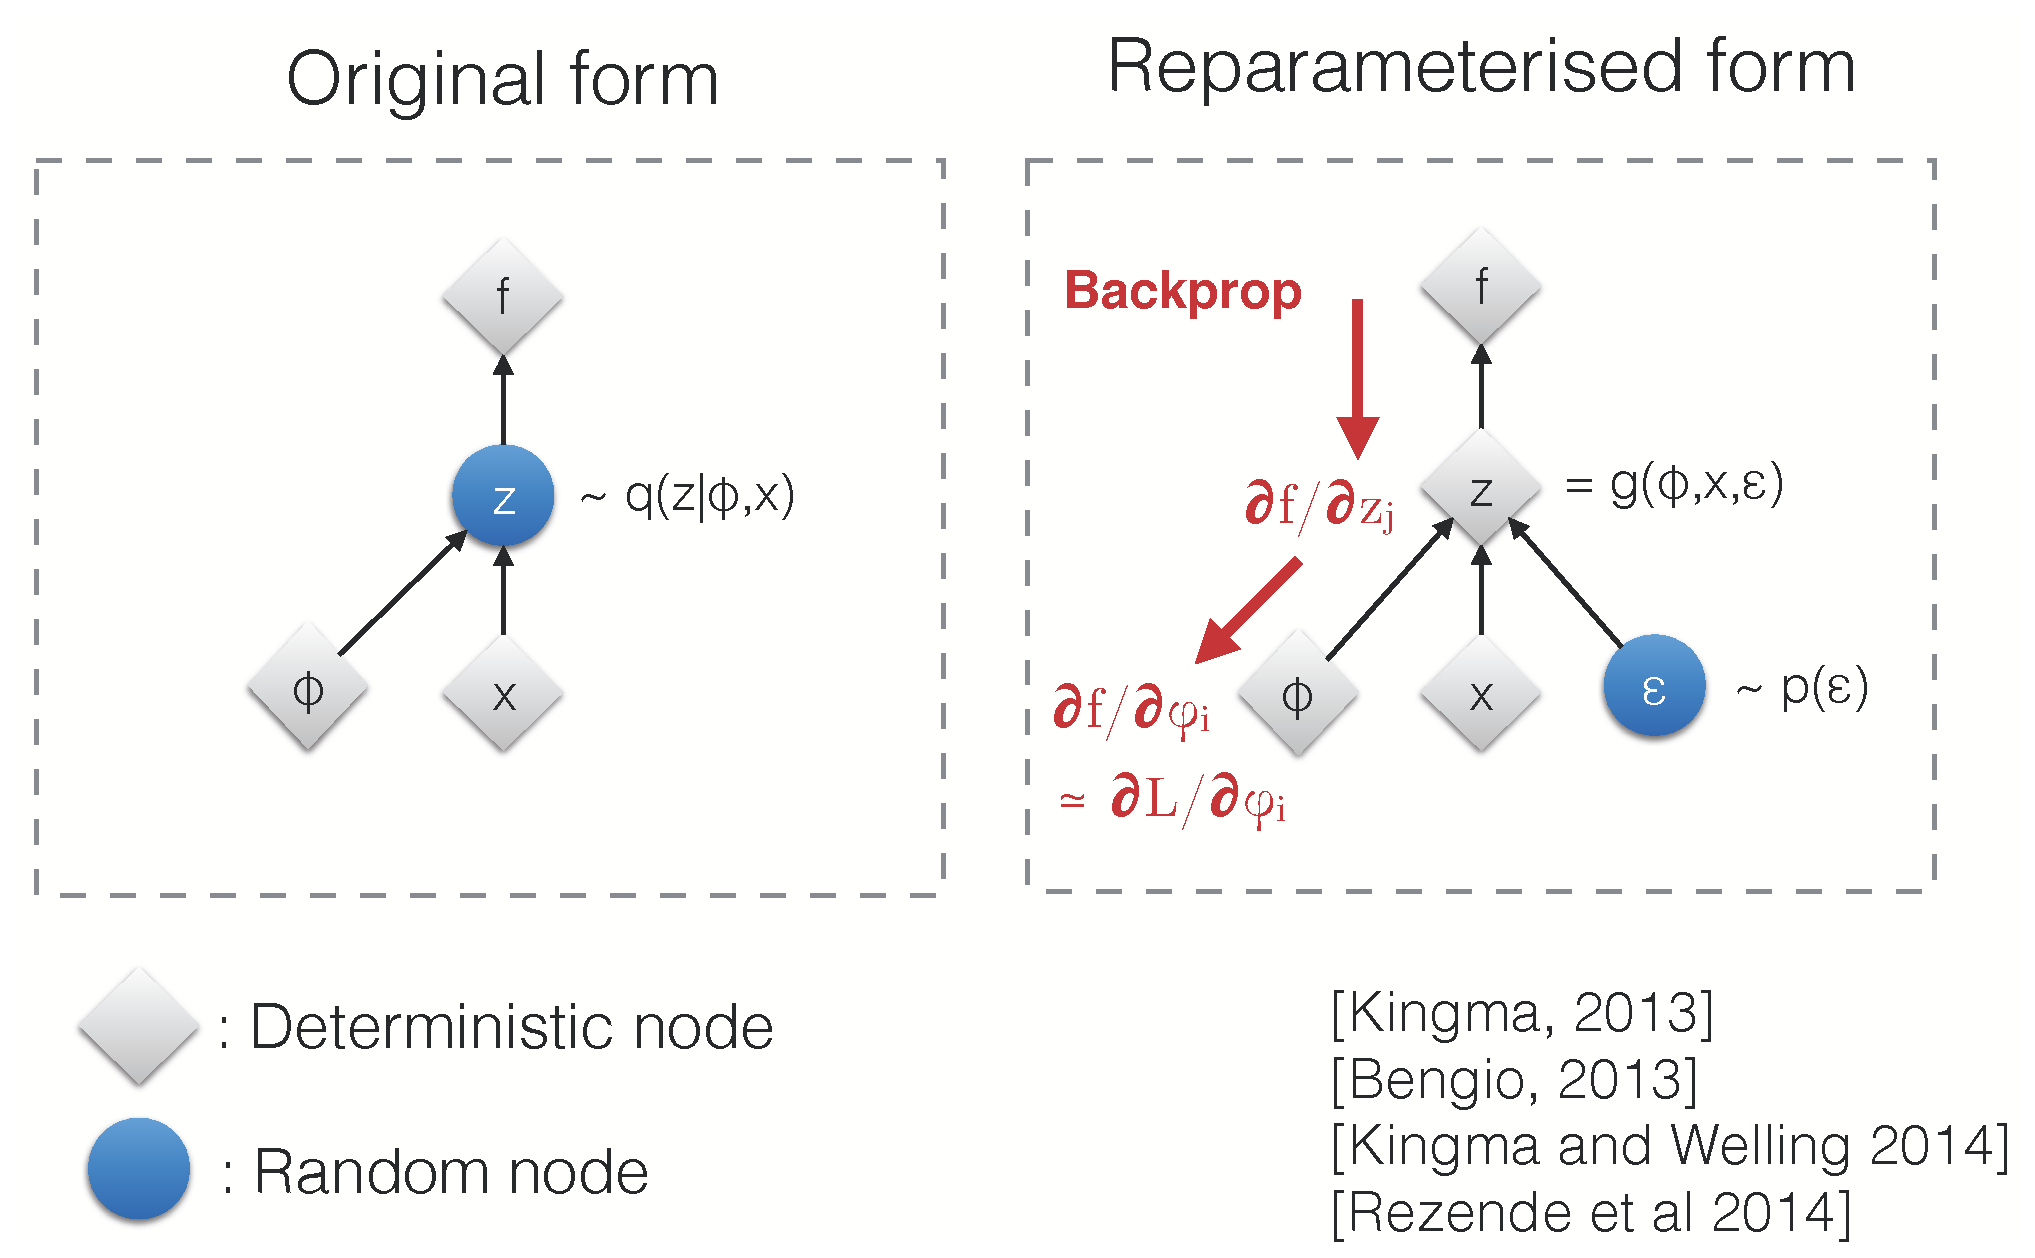
\includegraphics[width = 0.6\textwidth]{Reparameterization}
\end{figure}

假设$z$是服从以$\phi$和$x$为参数的分布$p(x|\phi, x)$,从该分布采样得到的$z$作为函数$f$的输入。由于$z$是采样得到的,故而不是确定的。所以在求导运算中便无法通过链式法则得到$\phi$和$x$的导数。reparameterization的技巧是通过将非确定节点移到运算树的叶节点上,从而可以应用链式法则求导。具体的做法是首先通过一个采样过程得到一个非确定的值$\varepsilon$,然后将$\varepsilon$同原始的参数$\phi$和$x$进行某种运算$g(\phi, x, \varepsilon)$得到$z$。

\section{Gaussian Reparameterization}
 如下图,在Variational Autoencoder模型中,我们需要将输入$x$编码为一个均值为$\mu$,方差为$\Sigma$的高斯分布然后从该高斯分布中采样一个隐变量$z$作为解码器的输入,该解码器将重构原始输入$x$。编码器和解码器可以是任意类型的神经网络。由于$z$是采样得到的不确定变量,所以在神经网络的训练过程中便无法使用反向传播来将梯度传给编码器。Reparameterization方法将该过程转换为给定输入$x$,编码器负责生成参数$\mu$和$\Sigma$,我们从标准正态分布中采样一个noise $\varepsilon$,然后通过$z=\mu + \Sigma*\varepsilon$得到需要的$z$。即,$\varepsilon$服从标准正太分布,则$z=\mu + \Sigma*\varepsilon$服从均值为$\mu$,方差为$\Sigma$的正太分布。令$F$为$z$的分布函数,则证明如下:
\begin{displaymath}
\begin{split}
F_z(x)&=P(z \leq x) = P(\mu + \Sigma*\varepsilon \leq x)=P(\varepsilon \leq \frac{x-\mu}{\Sigma}) = F_{\varepsilon}(\frac{x-\mu}{\Sigma})\\
f_Z(x) &= \frac{f_{\varepsilon}(\frac{x-\mu}{\Sigma})}{\Sigma} =\frac{1}{\sqrt{2\pi}\Sigma} exp \left\{ -\frac{(x-\mu)^2}{2 \Sigma^2} \right\} 
\end{split}
\end{displaymath}

\begin{figure}[htbp]
\centering
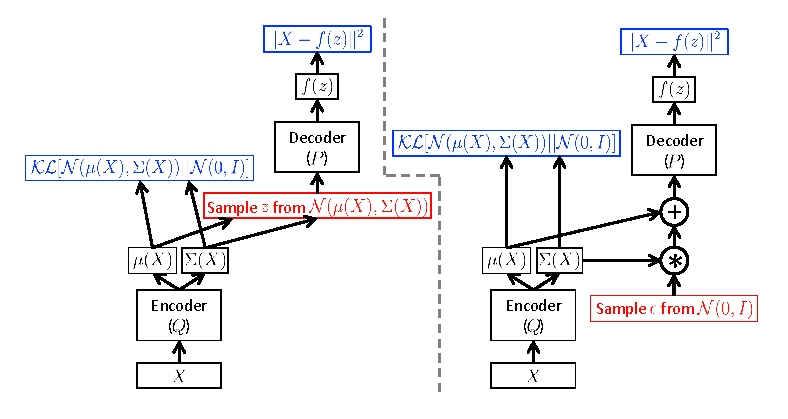
\includegraphics[width = 0.8\textwidth]{Vae_Reparameter}
\end{figure}

\section{Gumbel Max}

Gumbel Dsitribution 是定义在$(-\infty, +\infty)$之间的一个分布函数,定义如下:
\begin{displaymath}
p(x)=e^{-(x-\mu)-e^{-(x-\mu)}}
\end{displaymath}
其中$\mu$为一个均值参数,可以证明$p(x)$为一个概率分布。首先显然$e^{-(x-\mu)-e^{-(x-\mu)}}>0$,我们证明其和为1:

\begin{displaymath}
\begin{split}
\int_{-\infty}^{+\infty}p(x)\,\mathrm{d}x &=\int_{-\infty}^{+\infty}e^{-(x-\mu)-e^{-(x-\mu)}}\,\mathrm{d}x\\
&=\int_{-\infty}^{+\infty}e^{-x-e^{-x}}\,\mathrm{d}x\\
&\text{let } u=e^{-x}, \mathrm{d}u=-e^{-x}\mathrm{d}x=-u\mathrm{d}x\\
&=\int_{+\infty}^{0}-\frac{e^{\log{u}-e^{\log{u}}}}{u}\mathrm{d}u\\
&=\int_{+\infty}^{0}-e^{-u}\mathrm{d}u\\
&=\int_{0}^{+\infty}e^{u}\mathrm{d}u\\
&=1
\end{split}
\end{displaymath}

从而该分布的累计分布函数为: 
\begin{displaymath}
p(X \leqq x)=\int_{-\infty}^{x}e^{-(t-\mu)-e^{-(t-\mu)}}\mathrm{d}t =e^{-e^{-(x-\mu)}}
\end{displaymath}

在做多分类问题时,softmax通常被用来将多维的实数$[a_0, a_1, ... ,a_n]$映射为同样维度的概率分布$[p_0, p_1, ..., p_n]$, 其定义如下:
\begin{displaymath}
p(x)=\frac{e^{a_x}}{\sum_k{e^{a_k}}}
\end{displaymath}
有了这个$n$维的分布,我们便可以从该分布上采样。Gumbel Max则是用来将采样问题转化为一个优化问题。具体的,对于给定的一个softmax的分布,我们可以将每个$a_k$上加上一个$\mu=0$的Gumbel分布的noise,并取$argmax$,这样得到的最大值$k$遵从原来softmax的分布。

按此过程采样的结果为$x$,那么$x=k$的意思是对于$\forall k' \ne k, a_k + n_k \ge a_{k'} + n_{k'} $:
\begin{displaymath}
\begin{split}
p(x=k) &= \int ...\int{p(a_k + n_k \ge a_{k'} + n_{k'}, \forall k' \ne k)} \mathrm{d}n_1 ... \mathrm{d}n_K\\
&=\int p(n_k) \left[   \prod_{k' \neq k} \int p(a_k + n_k \ge a_{k'} + n_{k'}|n_k) \mathrm{d} n_{k}'  \right] \mathrm{d} n_k\\
&=\int p(n_k) \left[   \prod_{k' \neq k} \int p(n_{k'} \leq n_k + a_k - a_{k'}|n_k) \mathrm{d} n_{k}'  \right] \mathrm{d} n_k\\
&=\int p(n_k) \left[   \prod_{k' \neq k} e^{-e^{-(n_k+a_k-a_{k'})}}  \right] \mathrm{d} n_k\\
&=\int  e^{-n_k - e^{-n_k}} e^{-{\sum_{k \ne k'}{e^{-(n_k+a_k-a_{k'})}}}} \mathrm{d} n_k\\
&=\int  e^{-n_k - e^{-n_k}} e^{-e^{-n_k}(\sum_{k \ne k'}{e^{-(a_k-a_{k'})}})} \mathrm{d} n_k\\
&=\int  e^{-n_k - e^{-n_k}}e^{-e^{-n_k} (\sum_{k'}{e^{-(a_k-a_{k'})}})} \mathrm{d} n_k\\
\text{let } A &=\log \sum_{k'} e^{-(a_k-a_{k'})} = \log e^{-a_k} (\sum_{k'} e^{a_{k'}}) = \log{\sum_{k'} e^{a_{k'}}} -a_k:\\
&= \int e^{-n_k - e^{-n_k} - e^{-n_k  + A}} \mathrm{d} n_k\\
&=e^{-A} \int e^{-(n_k-A)-e^{-(n_k-A)}} \mathrm{d} n_k\\
&= e^{-A} = \frac{e^{a_k}}{\sum_{k'}{e^{a_{k'}}}}
\end{split}
\end{displaymath}




